\documentclass[11pt]{beamer}
\usetheme{Goettingen}
\usepackage[utf8]{inputenc}
\usepackage{amsmath}
\usepackage{amsfonts}
\usepackage{amssymb}
\usepackage{graphicx}
\usepackage{hyperref}
\author{Alex Heilman}
\title{Crystal Hypergraph Neural Networks}
\subtitle{A Universal Framework for Material Machine Learning}
%\setbeamercovered{transparent} 
%\setbeamertemplate{navigation symbols}{} 
%\logo{} 
%\institute{} 
%\date{} 
%\subject{} 

\newenvironment{boxed2}
    {\begin{center}
    \begin{tabular}{|p{0.95\textwidth}|}
    \hline\\
    }
    { 
    \\\\\hline
    \end{tabular} 
    \end{center}
    }


\begin{document}

\begin{frame}
\titlepage
\end{frame}

%\begin{frame}
%\tableofcontents
%\end{frame}

\begin{frame}{Overview}

$\bullet$ Crystal Graphs Lack Higher Order Geometrical Info of Crystal Structure \pause -- Motifs!

\vspace{.7cm}\pause

$\bullet$ Use Hypergraphs, with Motif Info/Shapes Encoded as Higher Order Hyperedge (Hedge) Attributes

\vspace{.7cm}\pause

$\bullet$ Convert Hypergraphs into 'Relatives' (Hetero) Graph  to Feed into Usual (Hetero) Graph Neural Networks, like CGCNN


\end{frame}

\section{Crystal Graphs}
\begin{frame}{Usual Crystal Graph Construction \small(a la CGCNN)}

$\bullet$ Atoms are nodes, with initial node features determined by atomic properties

\medskip

\begin{center}

\includegraphics[scale=0.3]{atom_feat.pdf}

\end{center}
\end{frame}

\begin{frame}{Crystal Graphs cont. I}

$\bullet$ Edges are determined by distance cutoff (4 Ang.) and maximum number of neighbors (12)

\begin{center}
\includegraphics[scale=0.45]{ex_bondcriteria.pdf}
\end{center}
\end{frame}

\begin{frame}{Crystal Graphs cont. II}
Edge attributes then are a Gaussian distance expansion

\begin{center}
\includegraphics[scale=0.33]{bond_feat.pdf}
\end{center}
\end{frame}

\begin{frame}{Graph Limitations}
Problem: Only encodes distances between atoms!

\vspace{.7cm}

Recent works: Atomistic Line graph generates a second graph (the line graph) associated with the crystal graph

\vspace{.4cm}

In line graph, nodes represent edges and line graph edges represent overlapping/connected edges.

\vspace{.4cm} 

Allows for encoding of angle information (between bonds) as edge attributes in line graph
\end{frame} 

\section{Crystal Hypergraphs}
\begin{frame}{Hypergraphs}
Hypergraphs allow us to have edges containing more than (or less than) two nodes.

\vspace{.5cm}

Natural way to encode features with higher order structure, where hypergraph nodes still represent atoms of underlying crystal structure.

\vspace{.5cm}

Can treat all different order structures on equal footing: each has a corresponding hyperedge with a feature
\end{frame}

\begin{frame}{Atom Hedges}
We first generate singleton hedges for each atomic site (the reason will be apparent later)

\vspace{0.5cm}

\begin{center}
\includegraphics[scale=0.73]{singleton.pdf}
\end{center}

\end{frame}

\begin{frame}{Pair Hedges}
Then generate pair (second order) hedges, equivalent to regular crystal graph edges.

\vspace{0.5cm}

\begin{center}
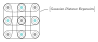
\includegraphics[scale=0.73]{pair.pdf}
\end{center}

\end{frame}

\begin{frame}{Motif Hedges}
Wish to include higher order geometrical information of crystal structure. Motifs have important information!

\vspace{0.5cm}\pause

Generate motif hedges, associate continuous symmetry measure for common motif shapes as feature.

\vspace{0.5cm}

\begin{center}
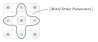
\includegraphics[scale=0.73]{motif.pdf}
\end{center}
\end{frame}



\section{Relatives Graph}
\begin{frame}
Next Problem: Current hypergraph convolution doesn't allow us to associate features with hyperedges!\pause

\vspace{.5cm}

Solution: Convert hypergraph into graph! \pause Then we can use the same graph networks previously developed (similar to Line graph's approach)

\vspace{.4cm}

Treat all order structures on equal footing; nodes for atoms, bonded atoms, motifs, and unit cell!

\vspace{.4cm}

Consider all order structures with common nodes connected (corresponding edge in relatives graph).
\end{frame}

\begin{frame}{Relatives Graph}
We term this inherited graph from the hypergraph the relatives graph, since connected nodes are related structures.
\begin{center}

\includegraphics[scale=0.33]{relgraph_workflow_horiz.pdf}
\end{center}

Note that this is naturally a heterogeneous graph, in that there are different types of nodes (can be projected into a homogeneous graph)
\end{frame}

\section{Current Results/Progress}
\begin{frame}
Important things to note:

\medskip

$\bullet$ CGConv performs much better than SAGEConv and TransformerConv (from Pytorch Geometric Library) on physical property tasks

\medskip

$\bullet$ Motif information shows substantial increase in performance even for underperforming convolutional structures on relatives graph
\end{frame}


\begin{frame}
Current Problems/Outlook:

\medskip

$\bullet$ CGConv (the most effective convolutional layer for such tasks) doesn't readily generalize

\medskip

$\bullet$ What other features/structure orders should be included?

\medskip

$\bullet$ What is the best balance between efficiency and efficacy?
\end{frame}

\end{document}